\section{Klasik Optimizasyon Algoritmalarının Teorik Temelleri}

Geleneksel optimizasyon yöntemleri, modern algoritmaların temel prensiplerini oluşturmakla kalmaz, aynı zamanda mühendislik problemlerinin çözümünde hala başvurulan en güvenilir araçlar arasındadır. Bu bölümde, bu yöntemlerin matematiksel altyapısına derinlemesine bir bakış sunacak ve yapısal optimizasyon problemlerine nasıl uygulandığını inceleyeceğiz.

\subsection{Matematiksel Optimizasyonun Analitik Temelleri}

Optimizasyon, matematik tarihi boyunca en köklü problemlerden biri olmuştur. Leibniz ve Newton'un diferansiyel hesabı geliştirmesinden önce bile matematikçiler optimizasyon problemleriyle uğraşmaktaydı. Modern anlamda matematiksel optimizasyonun analitik temelleri üç temel kavrama dayanır: stasyonerlik (durağanlık), konvekslik ve dualite.

\begin{tcolorbox}[title=Tarihsel Perspektif]
\begin{itemize}
    \item \textbf{Eski Yunan:} Öklidyen geometri ve maksimum-minimum problemleri
    \item \textbf{17. Yüzyıl:} Fermat, Leibniz ve Newton'un diferansiyel hesabı
    \item \textbf{18. Yüzyıl:} Lagrange ve Euler'in varyasyonel hesaplamaları
    \item \textbf{19. Yüzyıl:} Hamilton ve Jacobi'nin optimizasyon teorileri
    \item \textbf{20. Yüzyıl:} Doğrusal programlama, sayısal optimizasyon ve karmaşık algoritmaların gelişimi
\end{itemize}
\end{tcolorbox}

\subsubsection{Birinci ve İkinci Dereceden İyileştirme Koşulları}

Optimizasyonun matematiksel temelini oluşturan en önemli analitik koşullar şunlardır:

\textbf{Birinci Dereceden Gerek Koşul (Stasyonerlik):} 
Eğer $x^*$ noktası bir yerel minimum ise, $\nabla f(x^*) = 0$ olmalıdır. Bu, fonksiyonun gradyanının sıfır olduğu, yani teğet düzlemin yatay olduğu anlamına gelir.

\textbf{İkinci Dereceden Yeter Koşul:} 
Eğer $\nabla f(x^*) = 0$ ve Hessian matrisi $\nabla^2 f(x^*)$ pozitif tanımlı ise, $x^*$ bir kesin yerel minimumdur. Matematiksel olarak, tüm $d \neq 0$ için $d^T \nabla^2 f(x^*) d > 0$ koşulunun sağlanması gerekir.


\sidenote{İkinci dereceden koşullar, kritik noktanın (gradyanın sıfır olduğu nokta) yerel minimum, yerel maksimum veya eğer noktası olduğunu belirlememize yardımcı olur. Yapısal optimizasyon problemlerinde Hessian matrisinin değerlendirilmesi, algoritmanın ilerleyişi için kritik öneme sahiptir.}

\subsubsection{Konveks Optimizasyon Özel Durumu}

Konveks optimizasyon, klasik optimizasyon teorisinin özel bir durumudur ve dikkate değer özellikler taşır:

\begin{itemize}
    \item Amaç fonksiyonu ve kısıt kümesi konveks ise, her yerel minimum aynı zamanda global minimumdur
    \item Konveks problemlerde kritik nokta koşulları, global optimumu garanti eder
    \item Yapısal mekanikte doğrusal elastik yapıslar için potansiyel enerji minimizasyonu konveks bir problemdir
    \item Konveks olmayan problemler için bile, problem sıklıkla konveks alt problemlere ayrıştırılabilir
\end{itemize}

\begin{marginfigure}
\centering
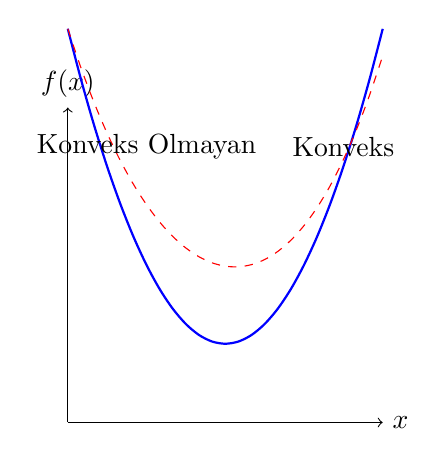
\begin{tikzpicture}
\draw[->] (0,0) -- (4,0) node[right] {$x$};
\draw[->] (0,0) -- (0,4) node[above] {$f(x)$};

% Konveks ve konveks olmayan fonksiyonlar
\draw[scale=1,domain=0:4,smooth,variable=\x,blue,thick] plot ({\x},{(\x-2)^2+1});
\node at (3.5,3.5) {Konveks};

\draw[scale=1,domain=0:4,smooth,variable=\x,red,dashed] plot ({\x},{sin(50*\x)+(\x-2)^2+1});
\node at (1,3.5) {Konveks Olmayan};

\end{tikzpicture}
\caption{Konveks ve konveks olmayan fonksiyonların karşılaştırması}
\label{fig:convexity}
\end{marginfigure}

\subsection{Gradyan Tabanlı Optimizasyon Algoritmaları}

Gradyan tabanlı algoritmalar, fonksiyonun türev bilgisini kullanarak sistematik bir şekilde optimum noktaya yaklaşan yöntemlerdir. Bu yöntemler, hesaplama verimliliği ve yakınsama özellikleri açısından yapısal optimizasyon problemlerinde büyük önem taşır.

\subsubsection{Gradyan İniş Yöntemi ve Varyasyonları}
Gradyan iniş yöntemi, en temel ve en eski gradyan tabanlı optimizasyon yöntemidir. Bu yöntem, fonksiyonun en hızlı azaldığı yönde ilerleyerek minimum noktaya ulaşmayı amaçlar.

\begin{equation}
x_{k+1} = x_k - \alpha_k \nabla f(x_k)
\end{equation}

Burada $\alpha_k$, adım boyutunu (veya öğrenme oranını) temsil eder ve algoritmanın performansını büyük ölçüde etkiler.

\begin{tcolorbox}[title=Gradyan İniş Varyasyonları]
\begin{itemize}
    \item \textbf{Sabit Adım Boyutu:} En basit yaklaşım, tüm iterasyonlarda sabit $\alpha$ kullanmaktır. Ancak hızlı yakınsama için çok düşük, stabilite için çok yüksek olabilir.
    
    \item \textbf{Line Search:} Her iterasyonda, $f(x_k - \alpha \nabla f(x_k))$ ifadesini minimize eden $\alpha_k$ değeri bulunur. Bu yaklaşım, Armijo, Wolfe veya Goldstein koşulları ile uygulanabilir.
    
    \item \textbf{Momentumlu Gradyan İniş:} Önceki gradyan değerlerini de dikkate alarak, yerel minimumlara takılmayı azaltır:
    $$x_{k+1} = x_k - \alpha_k \nabla f(x_k) + \beta (x_k - x_{k-1})$$
    
    \item \textbf{Nesterov Hızlandırılmış Gradyan:} Momentumlu gradyan inişin geliştirilmiş halidir, gradyanı mevcut konumda değil, momentumun götüreceği noktada hesaplar.
\end{itemize}
\end{tcolorbox}

\sidenote{Yapısal optimizasyon problemlerinde, gradyan iniş yöntemi genellikle büyük ölçekli problemlerin ilk aşamalarında kullanılır. Yakınsama hızı düşük olsa da, hesaplama maliyeti düşüktür ve karmaşık problemlerde iyi bir başlangıç noktası sağlayabilir.}

\begin{marginfigure}
\centering
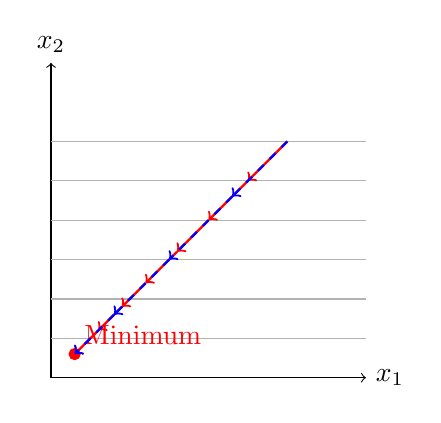
\begin{tikzpicture}
\draw[->] (0,0) -- (4,0) node[right] {$x_1$};
\draw[->] (0,0) -- (0,4) node[above] {$x_2$};

% Kontur çizgileri
\draw[scale=1,domain=0:4,smooth,variable=\x,black!30,thin] plot ({\x},{0.5});
\draw[scale=1,domain=0:4,smooth,variable=\x,black!30,thin] plot ({\x},{1.0});
\draw[scale=1,domain=0:4,smooth,variable=\x,black!30,thin] plot ({\x},{1.5});
\draw[scale=1,domain=0:4,smooth,variable=\x,black!30,thin] plot ({\x},{2.0});
\draw[scale=1,domain=0:4,smooth,variable=\x,black!30,thin] plot ({\x},{2.5});
\draw[scale=1,domain=0:4,smooth,variable=\x,black!30,thin] plot ({\x},{3.0});

% Gradyan iniş yolu
\draw[->,red,thick] (3,3) -- (2.5,2.5);
\draw[->,red,thick] (2.5,2.5) -- (2.0,2.0);
\draw[->,red,thick] (2.0,2.0) -- (1.6,1.6);
\draw[->,red,thick] (1.6,1.6) -- (1.2,1.2);
\draw[->,red,thick] (1.2,1.2) -- (0.9,0.9);
\draw[->,red,thick] (0.9,0.9) -- (0.6,0.6);
\draw[->,red,thick] (0.6,0.6) -- (0.3,0.3);
\filldraw[red] (0.3,0.3) circle (2pt) node[above right] {Minimum};

% Momentumlu gradyan iniş yolu
\draw[->,blue,thick,dashed] (3,3) -- (2.3,2.3);
\draw[->,blue,thick,dashed] (2.3,2.3) -- (1.5,1.5);
\draw[->,blue,thick,dashed] (1.5,1.5) -- (0.8,0.8);
\draw[->,blue,thick,dashed] (0.8,0.8) -- (0.3,0.3);

\end{tikzpicture}
\caption{Gradyan iniş (kırmızı, düz) ve momentumlu gradyan iniş (mavi, kesikli) yöntemlerinin karşılaştırması}
\label{fig:gradient_descent_variants}
\end{marginfigure}

\paragraph{Yapısal Optimizasyonda Gradyan Hesaplama}
Yapısal optimizasyon problemlerinde, gradyan hesaplama için genellikle üç yöntem kullanılır:

\begin{itemize}
    \item \textbf{Analitik Gradyan:} Doğrudan diferansiyel hesaplama ile elde edilir. En doğru sonucu verir ancak karmaşık sistemlerde türev çıkarımı zor olabilir.
    
    \item \textbf{Sonlu Farklar:} Sayısal yaklaşımla gradyan hesaplanır:
    $$\frac{\partial f}{\partial x_i} \approx \frac{f(x + h e_i) - f(x)}{h}$$
    Hesaplaması kolaydır ancak $h$ değerinin seçimi hassastır ve büyük sistemlerde hesaplama maliyeti yüksektir.
    
    \item \textbf{Adjoint Yöntemi:} Özellikle büyük ölçekli yapısal problemlerde verimlidir. Tasarım değişkeni sayısından bağımsız olarak sabit sayıda sistem çözümü gerektirir. Sonlu eleman analizlerinde sıklıkla kullanılır.
\end{itemize}

\subsubsection{Newton ve Quasi-Newton Yöntemleri}
Newton yöntemi, klasik optimizasyonun en güçlü araçlarından biridir. İkinci dereceden türev bilgisini (Hessian matrisini) kullanarak, fonksiyonun yerel kuadratik yaklaşımını oluşturur ve bu yaklaşımın minimum noktasına doğrudan ilerler.

\begin{equation}
x_{k+1} = x_k - [\nabla^2 f(x_k)]^{-1} \nabla f(x_k)
\end{equation}

Newton yönteminin en büyük avantajı, kuadratik yakınsama hızıdır; yani, optimum noktaya yaklaştıkça, hata her iterasyonda yaklaşık olarak karesi kadar azalır. Ancak, Hessian matrisinin hesaplanması ve tersinin alınması, özellikle yüksek boyutlu problemlerde hesaplama açısından maliyetlidir.

\paragraph{Modifiye Newton Yöntemleri}
Hesaplama maliyetini azaltmak ve Newton yönteminin kararsız olabileceği durumlarda daha iyi performans elde etmek için çeşitli modifikasyonlar geliştirilmiştir:

\begin{itemize}
    \item \textbf{Levenberg-Marquardt Algoritması:} Hessian matrisini, daha kararlı hale getirmek için modifiye eder:
    $$x_{k+1} = x_k - [\nabla^2 f(x_k) + \lambda I]^{-1} \nabla f(x_k)$$
    Burada $\lambda$, algoritmanın davranışını ayarlayan bir damping parametresidir.
    
    \item \textbf{Trust Region Newton Metodu:} Her iterasyonda, Hessian matrisinin geçerli olduğu bir "güvenilir bölge" tanımlar ve bu bölge içinde kuadratik modeli minimize eder. Özellikle yapısal optimizasyonda yaygın kullanılır.
\end{itemize}

\paragraph{Quasi-Newton Yöntemleri}
Tam Hessian matrisini hesaplama maliyetini ortadan kaldırmak için, quasi-Newton yöntemleri, Hessian matrisinin yaklaşık bir değerini iteratif olarak günceller. En popüler quasi-Newton yöntemleri şunlardır:

\begin{equation}
x_{k+1} = x_k - B_k^{-1} \nabla f(x_k)
\end{equation}

Burada $B_k$, Hessian matrisinin $k$. iterasyondaki yaklaşımıdır.

\begin{tcolorbox}[title=Temel Quasi-Newton Algoritmaları]
\begin{itemize}
    \item \textbf{BFGS (Broyden-Fletcher-Goldfarb-Shanno):} En yaygın kullanılan quasi-Newton yöntemidir. Hessian yaklaşımının pozitif tanımlılığını korur, bu da algoritmanın kararlılığını artırır. Yapısal optimizasyon problemlerinde sıklıkla tercih edilir.
    
    \item \textbf{DFP (Davidon-Fletcher-Powell):} BFGS'den daha eski bir yöntemdir, ancak genellikle BFGS kadar kararlı değildir.
    
    \item \textbf{SR1 (Symmetric Rank-One):} Daha az hesaplama gerektirir ancak pozitif tanımlılığı garanti etmez.
    
    \item \textbf{L-BFGS (Limited-memory BFGS):} Çok yüksek boyutlu problemler için geliştirilmiş, bellek kullanımı optimize edilmiş BFGS versiyonudur. Büyük ölçekli yapısal optimizasyon problemlerinde, özellikle topoloji optimizasyonunda tercih edilir.
\end{itemize}
\end{tcolorbox}

\paragraph{Yapısal Optimizasyonda Newton ve Quasi-Newton Uygulamaları}
Yapısal mühendislikte, Newton ve quasi-Newton yöntemleri şu tür problemlerde sıklıkla kullanılır:

\begin{itemize}
    \item \textbf{Şekil Optimizasyonu:} Yapının dış geometrisinin optimize edilmesinde, özellikle aerodinamik performans veya termal davranış için
    
    \item \textbf{Kesit Optimizasyonu:} Kafes ve çerçeve yapıların eleman kesitlerinin optimizasyonunda, özellikle doğrusal olmayan davranış gösteren yapılarda
    
    \item \textbf{Parametre Kalibrasyonu:} Sonlu eleman modellerinin deneysel verilerle kalibrasyonunda, malzeme parametrelerinin belirlenmesinde
    
    \item \textbf{Multi-fizik Optimizasyon:} Yapısal, termal ve akışkan davranışların birlikte optimize edildiği karmaşık mühendislik problemlerinde
\end{itemize}

\begin{marginfigure}
\centering
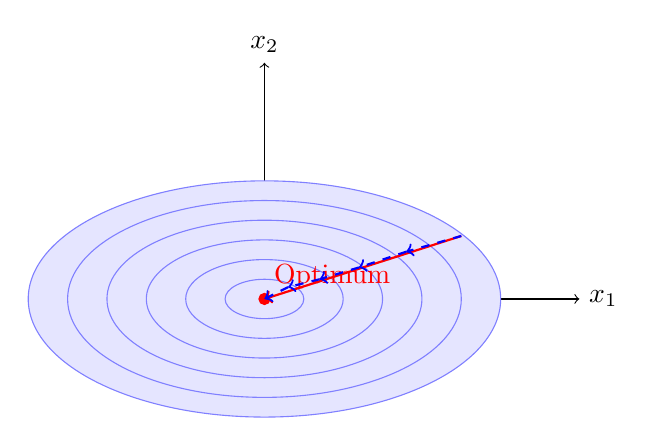
\begin{tikzpicture}
\draw[->] (0,0) -- (4,0) node[right] {$x_1$};
\draw[->] (0,0) -- (0,3) node[above] {$x_2$};

% Kontur çizgileri
\fill[blue!10] (0,0) ellipse (3 and 1.5);
\draw[blue!50] (0,0) ellipse (0.5 and 0.25);
\draw[blue!50] (0,0) ellipse (1 and 0.5);
\draw[blue!50] (0,0) ellipse (1.5 and 0.75);
\draw[blue!50] (0,0) ellipse (2 and 1);
\draw[blue!50] (0,0) ellipse (2.5 and 1.25);
\draw[blue!50] (0,0) ellipse (3 and 1.5);

% Newton yolu
\draw[->,red,thick] (2.5,0.8) -- (0,0);
\filldraw[red] (0,0) circle (2pt) node[above right] {Optimum};

% Gradyan iniş yolu
\draw[->,blue,thick,dashed] (2.5,0.8) -- (1.8,0.6);
\draw[->,blue,thick,dashed] (1.8,0.6) -- (1.2,0.4);
\draw[->,blue,thick,dashed] (1.2,0.4) -- (0.7,0.25);
\draw[->,blue,thick,dashed] (0.7,0.25) -- (0.3,0.15);
\draw[->,blue,thick,dashed] (0.3,0.15) -- (0,0);

\end{tikzpicture}
\caption{Newton yöntemi (kırmızı, düz) ve gradyan iniş yöntemi (mavi, kesikli) karşılaştırması. Newton yöntemi, kuadratik fonksiyonlarda tek adımda optimuma ulaşabilir.}
\label{fig:newton_vs_gradient}
\end{marginfigure}

\subsection{Kısıtlı Optimizasyon ve Dualite Teorisi}

Mühendislik problemleri nadiren kısıtsız olarak karşımıza çıkar. Yapısal tasarımda gerilme limitleri, deplasman sınırları, fiziksel kısıtlamalar ve kaynak sınırlamaları gibi pek çok kısıt söz konusudur. Bu bölümde, kısıtlı optimizasyon problemlerinin çözümüne yönelik klasik yaklaşımları derinlemesine inceleyeceğiz.

\subsubsection{Lagrange Çarpanları Yöntemi ve Teorik Temelleri}

Lagrange çarpanları yöntemi, eşitlik kısıtlı optimizasyon problemlerinin çözümü için geliştirilen temel bir yaklaşımdır. Joseph-Louis Lagrange'ın 18. yüzyılda geliştirdiği bu yöntem, optimizasyon teorisinin ve variasyonel hesaplamanın köşe taşlarından biridir.

Eşitlik kısıtlı bir optimizasyon problemi şu şekilde ifade edilir:
\begin{equation}
\begin{aligned}
\min & \quad f(x) \\
\text{s.t.} & \quad h_j(x) = 0, \quad j = 1, \ldots, p
\end{aligned}
\end{equation}

Lagrange fonksiyonu (veya Lagrangian) şu şekilde tanımlanır:
\begin{equation}
\mathcal{L}(x,\lambda) = f(x) + \sum_{j=1}^p \lambda_j h_j(x)
\end{equation}

Burada $\lambda_j$ değerleri, Lagrange çarpanları olarak adlandırılır ve her bir kısıtın "gölge fiyatını" veya marjinal değerini temsil eder.

\sidenote{Yapısal mühendislikte Lagrange çarpanları, çoğu zaman fiziksel bir anlam taşır. Örneğin, kuvvet dengesini kısıt olarak kullandığımız bir optimizasyon probleminde, Lagrange çarpanları genellikle yer değiştirmelere karşılık gelir. Bu dualite, sonlu eleman analizinde ve yapısal optimizasyonda temel bir kavramdır.}

\paragraph{Lagrange Koşulları}
Kısıtlı bir optimizasyon probleminin yerel minimumu için gerek koşullar şunlardır:

\begin{equation}
\begin{aligned}
\nabla_x \mathcal{L}(x^*,\lambda^*) &= \nabla f(x^*) + \sum_{j=1}^p \lambda_j^* \nabla h_j(x^*) = 0 \\
\nabla_{\lambda} \mathcal{L}(x^*,\lambda^*) &= h_j(x^*) = 0, \quad j = 1, \ldots, p
\end{aligned}
\end{equation}

Bu koşullar, optimal noktada amaç fonksiyonunun gradyanının, kısıt fonksiyonlarının gradyanlarının doğrusal bir kombinasyonuna eşit olması gerektiğini ifade eder. Geometrik olarak, bu, $f(x)$ ve $h_j(x)$ fonksiyonlarının seviye eğrilerinin teğet olması anlamına gelir.

\begin{figure}
\centering
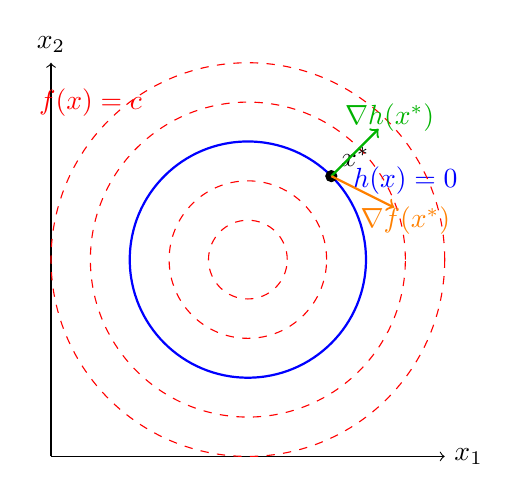
\begin{tikzpicture}
\draw[->] (0,0) -- (5,0) node[right] {$x_1$};
\draw[->] (0,0) -- (0,5) node[above] {$x_2$};

% Kısıt fonksiyonu (bir çember)
\draw[blue,thick] (2.5,2.5) circle (1.5);
\node[blue] at (4.5,3.5) {$h(x) = 0$};

% Amaç fonksiyonunun seviye eğrileri
\draw[red,dashed] (2.5,2.5) circle (0.5);
\draw[red,dashed] (2.5,2.5) circle (1);
\draw[red,dashed] (2.5,2.5) circle (2);
\draw[red,dashed] (2.5,2.5) circle (2.5);
\node[red] at (0.5,4.5) {$f(x) = c$};

% Optimum nokta
\filldraw[black] (3.56,3.56) circle (2pt) node[above right] {$x^*$};

% Gradyanlar
\draw[->,green!70!black,thick] (3.56,3.56) -- (4.16,4.16);
\node[green!70!black] at (4.3,4.3) {$\nabla h(x^*)$};

\draw[->,orange,thick] (3.56,3.56) -- (4.36,3.16);
\node[orange] at (4.5,3) {$\nabla f(x^*)$};

\end{tikzpicture}
\caption{Lagrange çarpanları yönteminin geometrik yorumu: Optimum noktada, amaç fonksiyonunun seviye eğrisi, kısıt fonksiyonunun seviye eğrisine teğettir.}
\label{fig:lagrange_geometry}
\end{figure}

\paragraph{İkinci Dereceden Koşullar}
Bir kritik noktanın gerçekten minimum olup olmadığını belirlemek için, genişletilmiş Hessian matrisinin incelenmesi gerekir. Eğer bu matris, kısıtların teğet uzayında pozitif tanımlı ise, kritik nokta bir yerel minimum olarak kabul edilir.

\begin{tcolorbox}[title=Lagrange Yönteminin Yapısal Optimizasyondaki Uygulamaları]
\begin{itemize}
    \item \textbf{Çelik Çerçeve Yapılar:} Ağırlık minimizasyonu yaparken, düğüm noktalarında kuvvet dengesi ve eleman uygunluğu kısıtlarının sağlanması
    
    \item \textbf{Kompozit Malzeme Tasarımı:} Rijitlik maksimizasyonu yaparken, hacim kısıtı ve malzeme dengesi koşullarının sağlanması
    
    \item \textbf{Kafes Sistemler:} Ağırlık minimizasyonu yaparken, izostatik denge koşullarının sağlanması
    
    \item \textbf{Sonlu Eleman Analizi:} Enerji minimizasyonu prensibine dayalı sonlu eleman formülasyonlarında, kinematik uygunluk ve kuvvet dengesi kısıtlarının sağlanması
\end{itemize}
\end{tcolorbox}

\subsubsection{Karush-Kuhn-Tucker (KKT) Koşulları ve Eşitsizlik Kısıtları}

Karush-Kuhn-Tucker (KKT) koşulları, Lagrange çarpanları yönteminin eşitsizlik kısıtlı problemlere genelleştirilmiş halidir. Bu koşullar, nonlineer programlama alanında optimum çözümlerin karakterizasyonu için temel bir çerçeve sunar.

Eşitsizlik kısıtlı bir optimizasyon problemi şu şekilde ifade edilir:
\begin{equation}
\begin{aligned}
\min & \quad f(x) \\
\text{s.t.} & \quad g_i(x) \leq 0, \quad i = 1, \ldots, m \\
& \quad h_j(x) = 0, \quad j = 1, \ldots, p
\end{aligned}
\end{equation}

Lagrange fonksiyonu bu durumda:
\begin{equation}
\mathcal{L}(x,\lambda,\mu) = f(x) + \sum_{i=1}^m \mu_i g_i(x) + \sum_{j=1}^p \lambda_j h_j(x)
\end{equation}

\paragraph{KKT Koşulları}
Eşitsizlik kısıtlı bir problemin yerel minimumu için gerekli koşullar (KKT koşulları) şunlardır:

\begin{equation}
\begin{aligned}
\nabla f(x^*) + \sum_{i=1}^m \mu_i^* \nabla g_i(x^*) + \sum_{j=1}^p \lambda_j^* \nabla h_j(x^*) &= 0 \\
g_i(x^*) &\leq 0, \quad i = 1, \ldots, m \\
h_j(x^*) &= 0, \quad j = 1, \ldots, p \\
\mu_i^* &\geq 0, \quad i = 1, \ldots, m \\
\mu_i^* g_i(x^*) &= 0, \quad i = 1, \ldots, m
\end{aligned}
\end{equation}

Son koşul "tamamlayıcı gevşeklik" olarak bilinir ve bir kısıtın ya aktif olması (eşitlik olarak sağlanması) ya da ilgili Lagrange çarpanının sıfır olması gerektiğini ifade eder.

\begin{tcolorbox}[title=KKT Koşullarının Yorumlanması]
\begin{itemize}
    \item \textbf{Stasyonerlik:} Amaç fonksiyonunun gradyanının, aktif kısıtların gradyanlarının doğrusal kombinasyonu olarak ifade edilmesi. Bu, optimum noktada ilerlemenin, en az bir aktif kısıtı ihlal etmeden mümkün olmadığını gösterir.
    
    \item \textbf{Uygunluk:} Tüm kısıtların sağlanması.
    
    \item \textbf{Çift Uygunluk:} Eşitsizlik kısıtları için Lagrange çarpanlarının (Kuhn-Tucker çarpanları) negatif olmaması. Bu, kısıtların yönünün önemli olduğunu gösterir.
    
    \item \textbf{Tamamlayıcı Gevşeklik:} Herhangi bir kısıt aktif değilse (eşitsizlik olarak sağlanıyorsa), ilgili Lagrange çarpanı sıfır olmalıdır. Bu, kısıtın "etkisiz" olduğu anlamına gelir.
\end{itemize}
\end{tcolorbox}

\paragraph{KKT Koşullarının Yapısal Optimizasyondaki Önemi}
Yapısal optimizasyon problemleri genellikle çok sayıda eşitsizlik kısıtı içerir. Örneğin:
\begin{itemize}
    \item Gerilme kısıtları: $\sigma_i \leq \sigma_{izin}$
    \item Deplasman kısıtları: $|u_i| \leq u_{izin}$
    \item Burkulma kısıtları: $P_i \leq P_{cr,i}$
    \item Geometrik kısıtlar: minimum kalınlık, genişlik vb.
\end{itemize}

Bu tür problemlerde, KKT koşulları sadece matematiksel bir araç değil, aynı zamanda fiziksel anlamı olan bir çerçeve sunar. Örneğin, gerilme kısıtına ait Lagrange çarpanı, ilgili noktada birim gerilme artışının, optimal tasarımın ağırlığına etkisini gösterir. Bu, "tasarım duyarlılığı analizi" için temel bir kavramdır.

\begin{marginfigure}
\centering
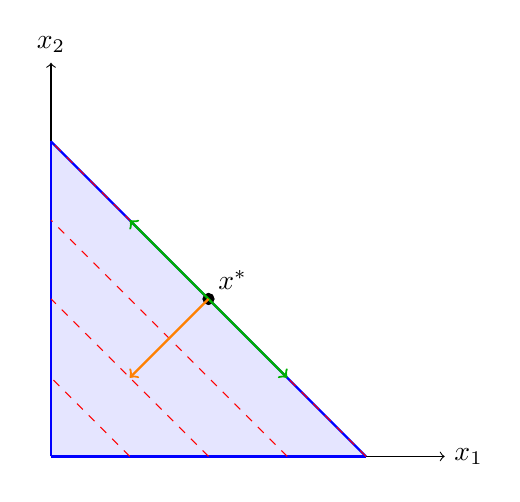
\begin{tikzpicture}
\draw[->] (0,0) -- (5,0) node[right] {$x_1$};
\draw[->] (0,0) -- (0,5) node[above] {$x_2$};

% Uygun bölge
\fill[blue!10] (0,0) -- (0,4) -- (2,2) -- (4,0) -- cycle;
\draw[blue,thick] (0,4) -- (2,2) -- (4,0);
\draw[blue,thick] (0,0) -- (0,4);
\draw[blue,thick] (0,0) -- (4,0);

% Amaç fonksiyonunun seviye çizgileri
\draw[red,dashed] (1,0) -- (0,1);
\draw[red,dashed] (2,0) -- (0,2);
\draw[red,dashed] (3,0) -- (0,3);
\draw[red,dashed] (4,0) -- (0,4);

% Optimum nokta
\filldraw[black] (2,2) circle (2pt) node[above right] {$x^*$};

% Aktif kısıtların gradyanları
\draw[->,green!70!black,thick] (2,2) -- (3,1);
\draw[->,green!70!black,thick] (2,2) -- (1,3);

% Amaç fonksiyonunun gradyanı
\draw[->,orange,thick] (2,2) -- (1,1);

\end{tikzpicture}
\caption{KKT koşullarının geometrik yorumu: Optimum noktada, amaç fonksiyonunun negatif gradyanı, aktif kısıtların gradyanlarının konveks konisinde yer alır.}
\label{fig:kkt_geometry}
\end{marginfigure}

\paragraph{Dualite Teorisi ve Ekonomik Yorum}
Lagrange dualitesi, birincil problem ile onun dual problemi arasındaki ilişkiyi inceler. Dual problem, birincil problemin Lagrange fonksiyonunun minimizasyonu yerine maksimizasyonunu içerir:

\begin{equation}
\begin{aligned}
\max_{\mu \geq 0, \lambda} \min_{x} \mathcal{L}(x,\lambda,\mu)
\end{aligned}
\end{equation}

Dualite teoremi, konveks bir birincil problem için, dual problemin optimal değerinin, birincil problemin optimal değerine eşit olduğunu ifade eder (güçlü dualite). Bu teorem, pek çok optimizasyon algoritmasının temelini oluşturur.

Ekonomik açıdan, dual değişkenler (Lagrange çarpanları) "gölge fiyatları" temsil eder. Yapısal optimizasyonda bu, bir kısıtın marjinal değişiminin, optimal tasarımın değerine etkisini gösterir. Bu yorum, mühendislere hangi kısıtların tasarım üzerinde en büyük etkiye sahip olduğunu anlama imkanı verir.

\begin{tcolorbox}[title=Dualite ve Yapısal Analiz Arasındaki İlişki]
Yapısal mekanikte, potansiyel enerji minimizasyonu (deplasman yöntemi) ve tamamlayıcı enerji minimizasyonu (kuvvet yöntemi) arasındaki ilişki, optimizasyon teorisindeki dualite kavramına mükemmel bir örnektir. 

Bir yapının analizi için:
\begin{itemize}
    \item \textbf{Birincil Problem (Deplasman Yöntemi):} Uyumlu deplasman alanını bulmak için potansiyel enerjiyi minimize etmek
    \item \textbf{Dual Problem (Kuvvet Yöntemi):} Dengedeki kuvvet dağılımını bulmak için tamamlayıcı enerjiyi minimize etmek
\end{itemize}

Bu dualite, yapısal optimizasyon algoritmalarının tasarımında da kullanılır. Özellikle "primal-dual" yöntemler, hem birincil hem de dual problemi eşzamanlı olarak çözerek, daha verimli optimizasyon sağlar.
\end{tcolorbox}

\subsection{Doğrusal ve Kuadratik Programlama}

Klasik optimizasyon yöntemlerinin önemli bir alt kümesi, doğrusal ve kuadratik programlama yöntemleridir. Bu yöntemler, belirli yapıdaki optimizasyon problemleri için özel olarak geliştirilmiş, verimli çözüm algoritmaları sunar.

\subsubsection{Doğrusal Programlama ve Yapısal Uygulamaları}

Doğrusal programlama (DP), hem amaç fonksiyonu hem de kısıtların doğrusal olduğu optimizasyon problemlerini inceler. Standart form:

\begin{equation}
\begin{aligned}
\min & \quad c^T x \\
\text{s.t.} & \quad Ax = b \\
& \quad x \geq 0
\end{aligned}
\end{equation}

Doğrusal programlama, 1940'larda George Dantzig'in Simplex algoritmasını geliştirmesiyle büyük bir ilerleme kaydetmiştir. Günümüzde, büyük ölçekli doğrusal programlama problemleri için İç Nokta Yöntemleri de yaygın olarak kullanılmaktadır.

\paragraph{Simplex Yöntemi ve Geometrik Yorumu}
Simplex yöntemi, uygun bölgenin köşe noktalarını (uç noktaları) sistematik olarak inceleyerek optimum çözümü bulmayı amaçlar. DP'nin temel teoremi, optimal çözümün uygun bölgenin bir köşe noktasında olması gerektiğini ifade eder (eğer çözüm tekil değilse).

Bu yöntemin adımları:
\begin{itemize}
    \item Başlangıç için bir uygun köşe noktası bulunur
    \item Amaç fonksiyonu değerini iyileştirecek komşu köşe noktasına geçilir
    \item Daha iyi bir komşu köşe bulunamayana kadar devam edilir
\end{itemize}



\begin{tcolorbox}[title=Yapısal Mühendislikte DP Uygulamaları]
\begin{itemize}
    \item \textbf{Plastik Limit Analizi:} Yapıların göçme yükünün belirlenmesi, plastik mafsal dağılımının optimizasyonu
    
    \item \textbf{Kafes Sistemlerin Minimum Ağırlık Tasarımı:} Eleman kesitlerinin optimizasyonunda, lineer davranış ve statik yük koşulları altında
    
    \item \textbf{Yapısal Kaynak Dağıtımı:} Sınırlı malzeme veya bütçe koşullarında, yapısal performansı maksimize edecek kaynak dağılımı
    
    \item \textbf{Ulaşım Ağı Optimizasyonu:} Köprü ve yol sistemlerinin yerleşiminin optimizasyonu, trafik akışının modellenmesi
\end{itemize}
\end{tcolorbox}

\paragraph{Plastik Limit Analizi Örneği}
Plastik limit analizi, doğrusal programlamanın yapısal mühendislikteki en önemli uygulamalarından biridir. Statik teorem (alt sınır) formülasyonu:
\begin{equation}
\begin{aligned}
\max & \quad \lambda \\
\text{s.t.} & \quad B^T q = \lambda F + F_0 \\
& \quad |q_i| \leq q_i^p, \quad i = 1, \ldots, n
\end{aligned}
\end{equation}

Burada:
\begin{itemize}
    \item $\lambda$: yük çarpanı
    \item $q$: iç kuvvetler vektörü
    \item $B$: denge matrisi
    \item $F$: değişken dış yük vektörü
    \item $F_0$: sabit dış yük vektörü
    \item $q_i^p$: eleman $i$ için plastik limit kapasitesi
\end{itemize}

Bu formülasyon, yapının göçmeden dayanabileceği maksimum yük çarpanını belirler.

\sidenote{Plastik limit analizi, özellikle çelik yapıların tasarımında önemlidir. Yapının elastik sınırın ötesinde, plastik deformasyon kapasitesini kullanarak dayanabildiği maksimum yükü belirleyerek, daha ekonomik tasarımlar elde edilmesini sağlar.}

\begin{marginfigure}
\centering
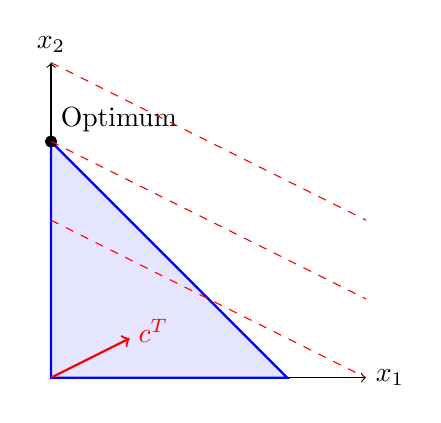
\begin{tikzpicture}
\draw[->] (0,0) -- (4,0) node[right] {$x_1$};
\draw[->] (0,0) -- (0,4) node[above] {$x_2$};

% Kısıtlar ve uygun bölge
\fill[blue!10] (0,0) -- (0,3) -- (1,2) -- (3,0) -- cycle;
\draw[blue,thick] (0,0) -- (0,3) -- (1,2) -- (3,0) -- cycle;

% Amaç fonksiyonu vektörü
\draw[->,red,thick] (0,0) -- (1,0.5);
\node[red] at (1.3,0.6) {$c^T$};

% Optimum nokta
\filldraw[black] (0,3) circle (2pt) node[above right] {Optimum};

% Amaç fonksiyonunun seviye çizgileri
\draw[red,dashed] (0,4) -- (4,2);
\draw[red,dashed] (0,3) -- (4,1);
\draw[red,dashed] (0,2) -- (4,0);

\end{tikzpicture}
\caption{Doğrusal programlamada uygun bölge ve optimum nokta}
\label{fig:linear_programming}
\end{marginfigure}

\subsubsection{Kuadratik Programlama}

Kuadratik programlama (KP), amaç fonksiyonunun ikinci dereceden, kısıtların ise doğrusal olduğu optimizasyon problemlerini ele alır:

\begin{equation}
\begin{aligned}
\min & \quad \frac{1}{2}x^TQx + c^Tx \\
\text{s.t.} & \quad Ax = b \\
& \quad x \geq 0
\end{aligned}
\end{equation}

Burada $Q$, simetrik bir matristir. Eğer $Q$ pozitif (yarı) tanımlı ise, problem konvekstir ve global optimumu bulmak göreceli olarak kolaydır.

\paragraph{Çözüm Yöntemleri}
Kuadratik programlama problemleri için çeşitli çözüm yöntemleri geliştirilmiştir:
\begin{itemize}
    \item \textbf{Aktif Set Yöntemleri:} Hangi kısıtların aktif olduğuna dair tahminler yaparak, kısıtsız optimizasyon alt problemlerini çözer
    
    \item \textbf{İç Nokta Yöntemleri:} Uygun bölgenin içinden geçerek, optimum noktaya yaklaşır
    
    \item \textbf{Sıralı Kuadratik Programlama (SQP):} Nonlineer optimizasyon problemlerini, kuadratik alt problemlere bölerek çözer
\end{itemize}



\begin{tcolorbox}[title=Yapısal Mühendislikte KP Uygulamaları]
\begin{itemize}
    \item \textbf{Elastik Deformasyon Minimizasyonu:} Yapının rijitlik matrisini kullanarak, belirli yükler altında deformasyonu minimize etmek
    
    \item \textbf{Dinamik Davranış Optimizasyonu:} Yapının kütle ve rijitlik matrislerini kullanarak, dinamik tepkiyi optimize etmek
    
    \item \textbf{Sonlu Eleman Modeli Kalibrasyonu:} Deneysel ve sayısal veriler arasındaki farkın karelerini minimize etmek
    
    \item \textbf{Ağırlık ve Deplasman Optimizasyonu:} Hem ağırlığı hem de deplasman enerjisini içeren çok amaçlı optimizasyon
\end{itemize}
\end{tcolorbox}

\paragraph{Yapısal Esneklik (Compliance) Minimizasyonu Örneği}
Yapısal tasarımda sıkça karşılaşılan bir kuadratik programlama problemi, belirli bir hacim kısıtı altında esnekliğin (veya deformasyon enerjisinin) minimizasyonudur:

\begin{equation}
\begin{aligned}
\min & \quad \frac{1}{2}F^Tu \\
\text{s.t.} & \quad Ku = F \\
& \quad \sum_{e=1}^{n_e} v_e\rho_e \leq V \\
& \quad 0 \leq \rho_e \leq 1, \quad e = 1, \ldots, n_e
\end{aligned}
\end{equation}

Burada:
\begin{itemize}
    \item $u$: deplasman vektörü
    \item $F$: kuvvet vektörü
    \item $K$: global rijitlik matrisi
    \item $\rho_e$: eleman $e$ için malzeme yoğunluğu (tasarım değişkeni)
    \item $v_e$: eleman $e$'nin hacmi
    \item $V$: izin verilen toplam hacim
\end{itemize}

Bu formülasyon, topoloji optimizasyonunun temelini oluşturur ve SIMP (Solid Isotropic Material with Penalization) metodunun başlangıç noktasıdır.

\subsection{Modern Klasik Optimizasyon Algoritmaları}

Klasik optimizasyon yöntemlerinin modern uzantıları, çeşitli yaklaşımlar kullanarak büyük ve karmaşık yapısal optimizasyon problemlerini çözmeyi amaçlar. Bu bölümde, klasik yöntemlerin daha gelişmiş versiyonlarını ele alacağız.

\subsubsection{Sekant Yöntemleri ve Yapısal Uygulamaları}

Sekant yöntemleri, Newton yönteminin Hessian matrisini hesaplama gereksinimini ortadan kaldırmak için geliştirilen yaklaşımlardır. Bu yöntemler, gradyan bilgisini kullanarak Hessian matrisinin yaklaşık bir tahminini oluşturur.

En yaygın sekant yöntemleri şunlardır:
\begin{itemize}
    \item \textbf{Broyden Yöntemi:} Genel nonlineer denklem sistemlerinin çözümünde kullanılır
    \item \textbf{DFP (Davidon-Fletcher-Powell) Yöntemi:} Quasi-Newton yöntemlerinin ilk örneklerindendir
    \item \textbf{BFGS (Broyden-Fletcher-Goldfarb-Shanno) Yöntemi:} Yapısal optimizasyon dahil birçok alanda standart haline gelmiştir
\end{itemize}

BFGS yönteminde, Hessian matrisinin yaklaşık değeri şu şekilde güncellenir:
\begin{equation}
B_{k+1} = B_k - \frac{B_k s_k s_k^T B_k}{s_k^T B_k s_k} + \frac{y_k y_k^T}{y_k^T s_k}
\end{equation}

Burada:
\begin{itemize}
    \item $s_k = x_{k+1} - x_k$
    \item $y_k = \nabla f(x_{k+1}) - \nabla f(x_k)$
\end{itemize}

BFGS yöntemi, yapısal optimizasyon problemlerinde, özellikle çok sayıda tasarım değişkeni söz konusu olduğunda yaygın kullanılır.

\paragraph{BFGS'in Yapısal Optimizasyondaki Avantajları}
\begin{itemize}
    \item \textbf{Bellek Verimliliği:} L-BFGS varyantı ile büyük ölçekli problemlerde bile uygulanabilir
    \item \textbf{Süper Lineer Yakınsama:} Optimum noktaya yaklaştıkça, yakınsama hızı artar
    \item \textbf{Sayısal Stabilite:} Newton yöntemine göre daha kararlıdır
    \item \textbf{Line Search ile Entegrasyon:} Güçlü line search stratejileriyle birleştirilebilir
\end{itemize}

\subsubsection{Trust Region ve Line Search Stratejileri}

Gradyan tabanlı optimizasyon yöntemlerinin performansı, adım boyutu seçimine büyük ölçüde bağlıdır. Line search ve trust region, adım boyutunu belirlemek için geliştirilen iki temel stratejidir.

\paragraph{Line Search Stratejileri}
Line search yöntemlerinde, arama yönü $d_k$ belirlendikten sonra, uygun adım boyutu $\alpha_k$ bulunur:
\begin{equation}
x_{k+1} = x_k + \alpha_k d_k
\end{equation}

Optimal adım boyutunu belirlemek için çeşitli kriterler kullanılır:
\begin{itemize}
    \item \textbf{Armijo Koşulu:} Adım boyutunun, fonksiyon değerinde yeterli azalma sağlamasını garantiler
    \item \textbf{Wolfe Koşulları:} Armijo koşuluna ek olarak, gradyan değişiminin belirli bir oranı sağlamasını gerektirir
    \item \textbf{Goldstein Koşulları:} Hem fonksiyon değerinde azalma hem de adım boyutunun çok küçük olmamasını sağlar
\end{itemize}

\paragraph{Trust Region Yaklaşımı}
Trust region yöntemlerinde, modelin güvenilir olduğu bir bölge tanımlanır ve bu bölge içinde model minimize edilir:
\begin{equation}
\begin{aligned}
\min & \quad m_k(p) = f_k + g_k^Tp + \frac{1}{2}p^TB_kp \\
\text{s.t.} & \quad \|p\| \leq \Delta_k
\end{aligned}
\end{equation}

Burada:
\begin{itemize}
    \item $m_k(p)$: $k$. iterasyonda fonksiyonun kuadratik modeli
    \item $f_k = f(x_k)$, $g_k = \nabla f(x_k)$
    \item $B_k$: Hessian matrisi veya yaklaşımı
    \item $\Delta_k$: trust region yarıçapı
\end{itemize}

Her iterasyonda, model tahmini ile gerçek fonksiyon değişimi karşılaştırılarak, trust region yarıçapı güncellenir.

\begin{tcolorbox}[title=Yapısal Mühendislikte Trust Region Uygulamaları]
Trust region yaklaşımı, yapısal mühendislikte özellikle şu durumlarda tercih edilir:
\begin{itemize}
    \item \textbf{Kötü Koşullu Problemler:} Rijitlik matrisinin koşul sayısının yüksek olduğu durumlarda
    \item \textbf{Doğrusal Olmayan Davranış:} Malzeme veya geometrik nonlineerite içeren yapısal analizlerde
    \item \textbf{Kararsız Sistemler:} Burkulma analizi gibi kararsızlık noktalarına yakın problemlerde
    \item \textbf{Çoklu Fizik Analizleri:} Termal-yapısal, akışkan-yapı etkileşimi gibi karmaşık multifizik problemlerde
\end{itemize}
\end{tcolorbox}

\subsubsection{Sıralı Kısıt Programlama}

Sıralı Kısıt Programlama (Sequential Constraint Programming - SCP), yapısal optimizasyon problemlerinin çözümü için geliştirilen etkili bir yaklaşımdır. Bu yöntem, nonlineer problemi, bir dizi doğrusal alt probleme dönüştürerek çözer.

SCP'nin temel yaklaşımı:
\begin{itemize}
    \item Nonlineer kısıtları, mevcut iterasyon noktası etrafında doğrusallaştırır
    \item Doğrusallaştırılmış problemi çözer
    \item Çözümü yeni bir iterasyon noktası olarak kullanır
    \item Yakınsama sağlanana kadar tekrarlar
\end{itemize}

Bu yöntem, MMA (Method of Moving Asymptotes) gibi daha gelişmiş varyantlarıyla, yapısal topoloji optimizasyonunda yaygın olarak kullanılmaktadır.


MMA'nın yapısal optimizasyondaki başlıca avantajları:
\begin{itemize}
    \item Büyük ölçekli topoloji optimizasyonu problemlerinde verimlilik
    \item Doğrusal olmayan kısıtları etkin bir şekilde ele alabilme
    \item Salınımları azaltarak kararlı yakınsama sağlama
    \item Paralel hesaplamaya uygunluk
\end{itemize}

\begin{figure}
\centering
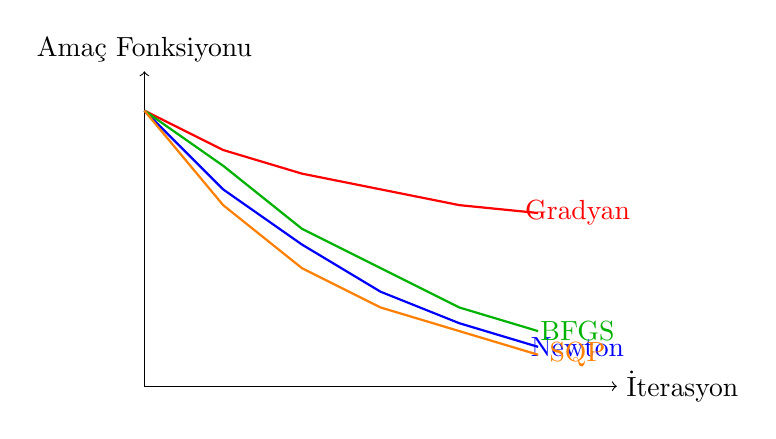
\begin{tikzpicture}
\draw[->] (0,0) -- (6,0) node[right] {İterasyon};
\draw[->] (0,0) -- (0,4) node[above] {Amaç Fonksiyonu};

% Gradyan iniş
\draw[red,thick] plot coordinates {(0,3.5) (1,3.0) (2,2.7) (3,2.5) (4,2.3) (5,2.2)};
\node[red] at (5.5,2.2) {Gradyan};

% Newton
\draw[blue,thick] plot coordinates {(0,3.5) (1,2.5) (2,1.8) (3,1.2) (4,0.8) (5,0.5)};
\node[blue] at (5.5,0.5) {Newton};

% BFGS
\draw[green!70!black,thick] plot coordinates {(0,3.5) (1,2.8) (2,2.0) (3,1.5) (4,1.0) (5,0.7)};
\node[green!70!black] at (5.5,0.7) {BFGS};

% SQP
\draw[orange,thick] plot coordinates {(0,3.5) (1,2.3) (2,1.5) (3,1.0) (4,0.7) (5,0.4)};
\node[orange] at (5.5,0.4) {SQP};

\end{tikzpicture}
\caption{Farklı optimizasyon algoritmalarının yakınsama davranışlarının karşılaştırması}
\label{fig:convergence_comparison}
\end{figure}

\subsection{Sonuç ve Modern Yöntemlere Geçiş}

Klasik optimizasyon yöntemleri, yapısal mühendislikte karşılaşılan çeşitli problemlerin çözümünde hala büyük önem taşımaktadır. Bu yöntemler, modern meta-sezgisel algoritmaların ve yapay zeka tabanlı yaklaşımların temelini oluşturur.

\begin{tcolorbox}[title=Klasik ve Modern Yöntemlerin Karşılaştırması]
\begin{itemize}
    \item \textbf{Klasik Yöntemler:} Matematiksel sağlamlık, kesin yakınsama garantileri, verimlilik
    \item \textbf{Modern Yöntemler:} Çok modlu fonksiyonlar için global arama, paralel hesaplama, karmaşık kısıtların ele alınmasında esneklik
\end{itemize}
\end{tcolorbox}

Günümüzde, klasik algoritmaların güçlü yönleri ile modern yaklaşımların esnekliğini birleştiren hibrit yöntemler büyük ilgi görmektedir. Bu hibrit yaklaşımlar, özellikle büyük ölçekli ve çok amaçlı yapısal optimizasyon problemlerinde etkili çözümler sunmaktadır.
